\subsection{Metal Bare}
برای قسمت
\lr{bare metal}
دقیقا کانفیگ
\lr{PostgreSQL}
را با 16
\lr{warehouse}
و 2 کاربر را وارد
\lr{hammerdb}
می‌کنیم. به کمک دستورات زیر نیز
\lr{MySQL}
را بنچمارک می‌کنیم. فقط حواستان باشد که در دستور
\lr{strace}
به کمک آپشن
\codeword{-e}
دو فراخوانی سیستمی
\lr{futex} و \lr{io\_getevents}
را از لاگ حذف کردیم.
\codebox{
    perf record -p \$(pidof mysqld | tr ' ' ',') -o hammerdb-schema-build-bare-metal-5.perf -e tlb:tlb\_flush,dTLB-loads,dTLB-load-misses,iTLB-load-misses,cache-misses,page-faults\\
    strace -f -p "\$(pidof mysqld)" -e 'trace=!futex,io\_getevents' 2> hammerdb-schema-build-bare-metal-5.strace
}
در ابتدا مانند قسمت
\lr{PostgreSQL}
باید
\lr{schema}
را بسازیم. من بر روی کرنل نسخه‌ی 5 که توسط خود
\lr{Ubuntu}
نصب شده بود
\lr{schema}
را ساختم و در تمامی مراحل ساخت به کمک
\lr{perf} و \lr{strace}
کارکرد
\lr{MySQL}
را زیر نظر گرفتم. قسمتی از ساخت
\lr{schema}
را می‌توانید در شکل
\ref{fig:mysql:baremetal:schema}
مشاهده کنید.
\begin{figure}[H]
    \centering
    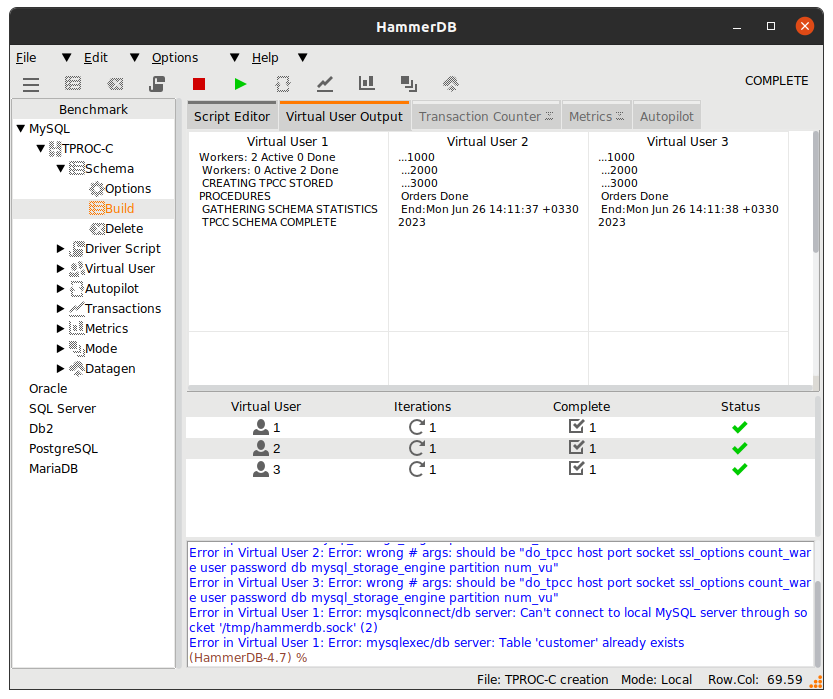
\includegraphics[scale=0.5]{pictures/mysql/baremetal/schema-build.png}
    \caption{ساخت \lr{schema} در محیط \lr{bare metal}}
    \label{fig:mysql:baremetal:schema}
\end{figure}
در ادامه با تنظیم کردن پارامتر‌های بنچمارک، بنچمارک اصلی را انجام دادیم.
مانند
\lr{PostgreSQL}
ما 3 دقیقه برای
\lr{warmup}
و 7 دقیقه برای تست اصلی در نظر گرفتیم. سپس بنچمارک را برای ورژن‌های مختلف کرنل لینوکس انجام دادیم.
(شکل \ref{fig:mysql:baremetal:benchmark})
\begin{figure}[H]
    \centering
    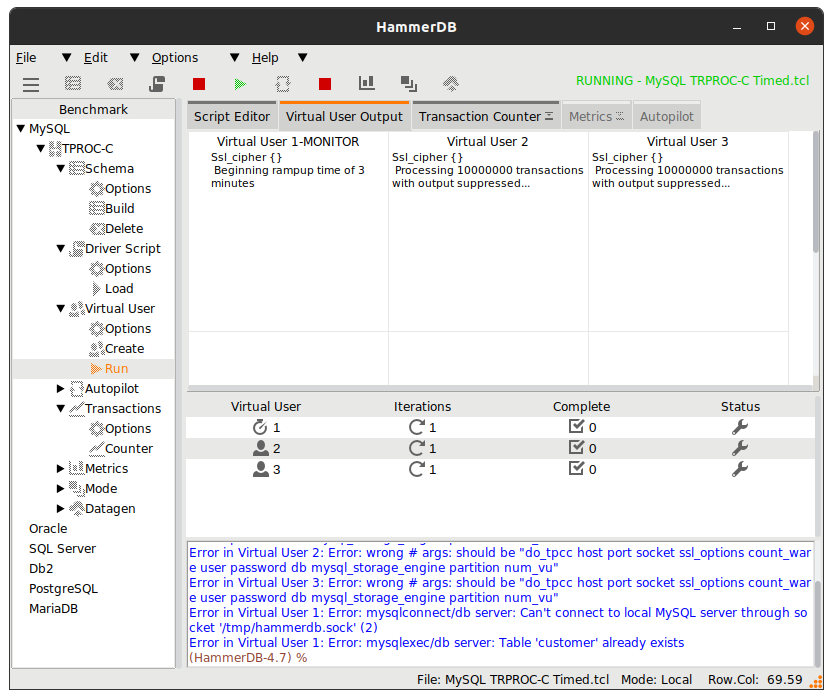
\includegraphics[scale=0.5]{pictures/mysql/baremetal/benchmark-1.png}
    \caption{\lr{benchmark} در محیط \lr{bare metal}}
    \label{fig:mysql:baremetal:benchmark}
\end{figure}
همچنین سایز دیتابیس را مشاهده می‌کنیم که در شکل
\ref{fig:mysql:baremetal:dbsize}
آمده است.
\begin{figure}[H]
    \centering
    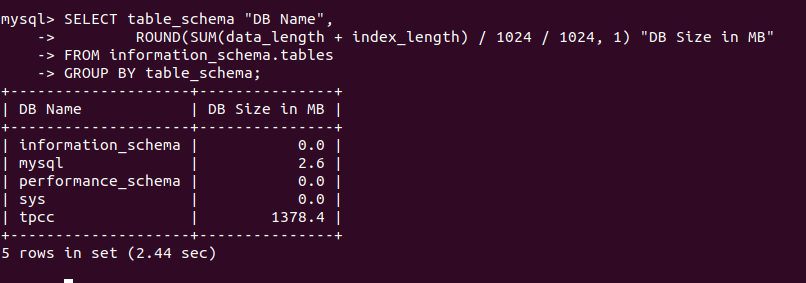
\includegraphics[scale=0.5]{pictures/mysql/baremetal/db-size.png}
    \caption{حجم دیتابیس}
    \label{fig:mysql:baremetal:dbsize}
\end{figure}
یکی از نکاتی که در
\lr{MySQL}
دیدم،
\lr{TPM}
به شدت پایین‌تر نسبت به
\lr{PostgreSQL}
و همچنین بی‌نهایت پر نوسان‌تر بود. به عنوان مثلا در شکل
\ref{fig:mysql:baremetal:tpm}
می‌توانید دو نمونه از سرعت‌ها را نگاه کنید. با توجه به تحقیقات و مشاهدات بیشتری که انجام دادیم متوجه
شدیم که در قسمت
\lr{warmup}، \lr{TPM}
در حدود 900 و در قسمت
\lr{real benchmark}
در حدود 350 است که افت بسار عجیبی است.
\begin{figure}[H]
    \centering
    \centering
    \subfloat[TPM در ابتدای تست]{{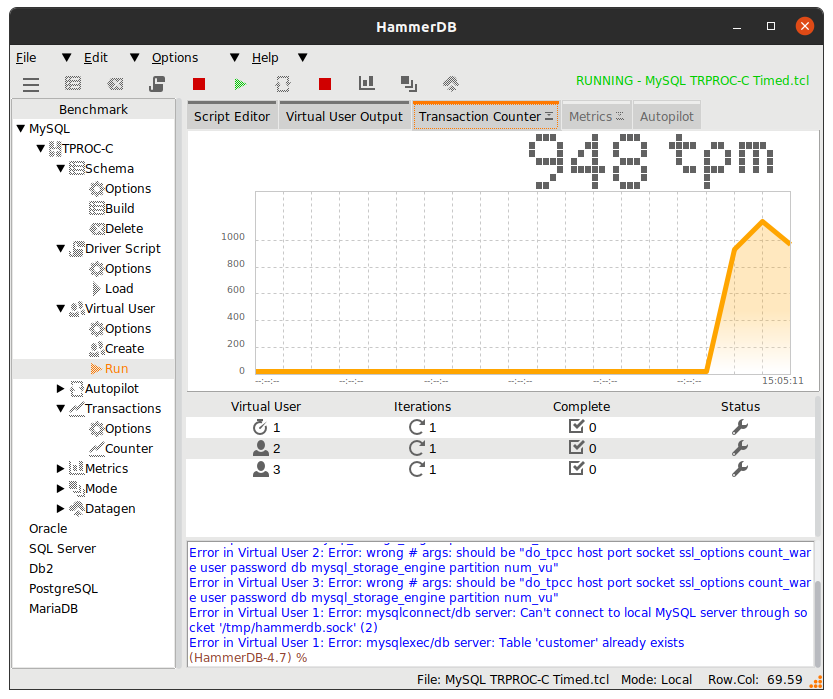
\includegraphics[scale=0.2]{pictures/mysql/baremetal/benchmark-tpm1.png}}}
    \quad
    \subfloat[TMP در انتهای تست]{{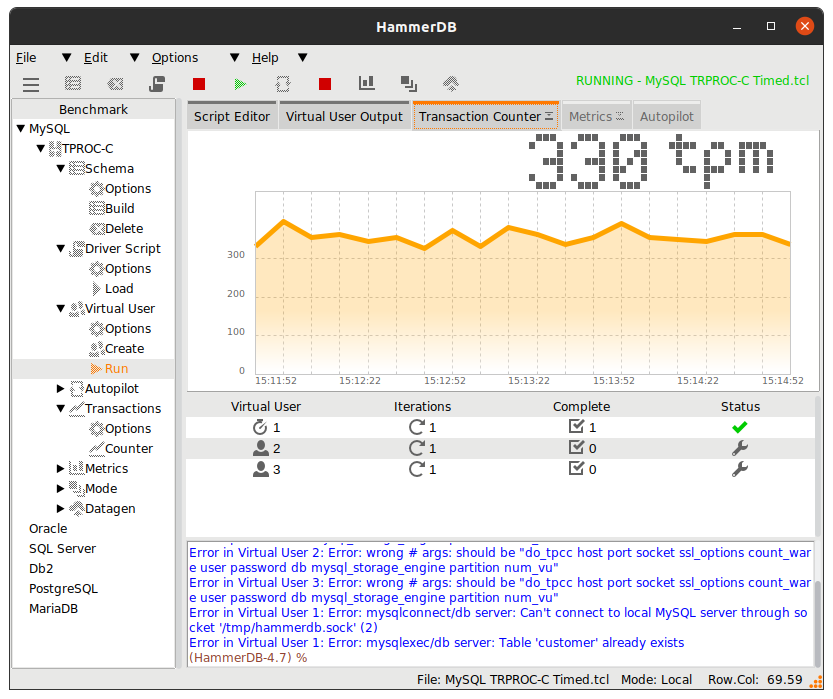
\includegraphics[scale=0.2]{pictures/mysql/baremetal/benchmark-tpm2.png}}}
    \caption{\lr{TPM} در محیط \lr{bare metal}}
    \label{fig:mysql:baremetal:tpm}
\end{figure}
